

\documentclass[../analysis1.tex]{subfiles}

\begin{document}




\chapter{Convergence of Functions}

In the last chapter, we implicitly introduced the notion of convergence of \textit{functions} to \textit{other functions}, during our discussion of Taylor series, which are a very particular type of function sequence (polynomials). This was a concept called \textit{pointwise convergence}, as we will define properly below, and the results we proved were \textit{pointwise} results. This motivates a more general study of convergence of functions, which we will discuss in this chapter.

\section{Pointwise Convergence}

\begin{definition}[Pointwise Convergence]
    \begin{shaded*}
        A sequence of functions $f_n: D \to \R$ converges \textit{pointwise} to a limit function $f : D \to \R$ if, for every $x \in D$, the sequence of real numbers $(f_n(x))_{n=1}^\infty$ converges to $f(x)$.
        In such a case, we may write $f_n\to f$ pointwise.
        
    \end{shaded*}
\end{definition}
\begin{remark}
    In quantifiers, this definition translates to:
    \[\forall x \in D,\,\forall \varepsilon > 0,\, \exists N\in\N,\, \forall n \ge N,\, |f_n(x) - f(x)| < \varepsilon.\]
    Notice that $N$ may depend on \textit{both} the point $x$ \textit{and} $\varepsilon$, i.e. we may write $N=N(x,\varepsilon)$. It is helpful to keep the following picture in mind:
\end{remark}


\begin{center}
    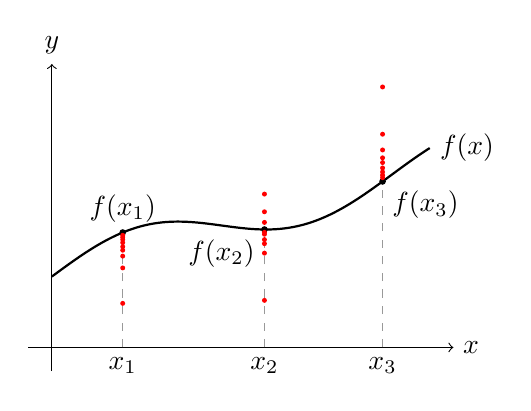
\begin{tikzpicture}[
        declare function={
            f(\x) = 0.5*sin(\x * 50) + 0.3*\x + 1.5;
        }, scale=0.6
    ]
        % Axes
        \draw[->] (-0.5, 0) -- (8.5, 0) node[right] {$x$};
        \draw[->] (0, -0.5) -- (0, 6.0) node[above] {$y$};
    
        \draw[thick, domain=0:8, samples=100] plot (\x, {f(\x)}) node[right] {$f(x)$};
    
        
        \def\xone{1.5}
        \draw[dashed, gray!80] (\xone, 0) node[below, text=black] {$x_1$} -- (\xone, {f(\xone)});
        
        \fill[black] (\xone, {f(\xone)}) circle (2pt) node[above] {$f(x_1)$};
        
        \foreach \n in {1, 2, 3, 4, 5, 7, 10, 15, 25} {
            \fill[red] (\xone, {f(\xone) - 1.5/\n}) circle (1.5pt);
        }
    
    
        \def\xtwo{4.5}
        \draw[dashed, gray!80] (\xtwo, 0) node[below, text=black] {$x_2$} -- (\xtwo, {f(\xtwo)});
        
        \fill[black] (\xtwo, {f(\xtwo)}) circle (2pt) node[below left] {$f(x_2)$};
        
        \foreach \n in {1, 2, 3, 4, 5, 7, 10, 15, 25} {
            \fill[red] (\xtwo, {f(\xtwo) + 1.5*cos(\n*180)/\n}) circle (1.5pt);
        }
    
    
        \def\xthree{7}
        \draw[dashed, gray!80] (\xthree, 0) node[below, text=black] {$x_3$} -- (\xthree, {f(\xthree)});
        
        \fill[black] (\xthree, {f(\xthree)}) circle (2pt) node[below right] {$f(x_3)$};
        
        \foreach \n in {1, 2, 3, 4, 5, 7, 10, 15, 25} {
            \fill[red] (\xthree, {f(\xthree) + 2/\n}) circle (1.5pt);
        }
        
    
    \end{tikzpicture}
\end{center}

As illustrated above, pointwise convergence means that for every $x$ in the domain, we have a different limit $\lim_{n\to\infty}f_n(x)$ that converges to some value $f(x)$ (where $f$ is the limit function). For example, if the domain of each $f_n$ is the open interval $(0,1)$, then we have uncountably many limits to consider.


Pointwise convergence is a weak notion of function convergence because it evaluates the limit completely independently for each isolated coordinate $x$. It treats a function sequence merely as an unlinked collection of individual point-sequences rather than a cohesive geometric object.

To make these issues concrete, we examine how pointwise convergence can destroy both continuity and integrability.

\begin{example}
    Consider the sequence $f_n(x) = x^n$ on the interval $[0,1]$. Each function in the sequence is continuous. Pointwise evaluation yields the discontinuous step function (by standard properties of the limit from Chapter 2):
    \[
        f(x) = \lim_{n \to \infty} f_n(x) = \begin{cases} 0, & x \in [0,1), \\ 1, & x = 1. \end{cases}
    \]
    \begin{center}
    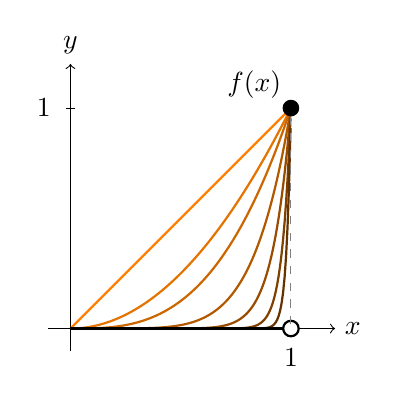
\begin{tikzpicture}[scale=2.8]
        % Axes
        \draw [->] (-0.1, 0) -- (1.2, 0) node [right] {$x$};
        \draw [->] (0, -0.1) -- (0, 1.2) node [above] {$y$};
      
        \begin{scope}
          \clip (-0.1, -0.1) rectangle (1.2, 1.2);
      
          % Sequence of functions f_n(x) = x^n
          % \i controls the color shading, \n is the exponent
          \foreach \i/\n in {
            0/1, 
            1/2, 
            2/3, 
            3/6, 
            4/12, 
            5/25, 
            6/50
          } {
            \pgfmathsetmacro\c{100 - 10 * \i};
            
            \draw [domain=0:1, samples=150, orange!\c!black, thick] 
              plot (\x, {\x^\n});
          }
        \end{scope}
      
        % Ticks
        \draw (1, 0.02) -- (1, -0.02) node [below=2pt] {$1$};
        \draw (0.02, 1) -- (-0.02, 1) node [left=2pt] {$1$};
      
        % Limit function f(x)
        % Bridged cleanly across the discontinuity
        
        % Limit function for x in [0, 1)
        \draw [thick, black] (0, 0) -- (1, 0);
        % Open circle at (1, 0) to indicate the limit function is 0 strictly before 1
        \filldraw [fill=white, draw=black, thick] (1, 0) circle (1pt);
      
        % Dashed line to highlight the discontinuous jump
        \draw [dashed, gray] (1, 0.02) -- (1, 0.98);
      
        % Limit function at x = 1
        \filldraw [black] (1, 1) circle (1pt) node [above left] {$f(x)$};
      
      \end{tikzpicture}
    \end{center}
    To force the function values to drop below an error threshold $\varepsilon > 0$ for $x \in (0,1)$, we require $x^n < \varepsilon$, which dictates our choice of $N$:
    \[
        N = \left\lceil \frac{\log \varepsilon}{\log x} \right\rceil.
    \]
    Notice that as $x$ approaches $1$ from the left, $\log x \to 0$, forcing $N \to \infty$. The convergence becomes arbitrarily slow near the boundary. 
    
    This shows precisely why the pointwise convergence does not guarantee continuity in the limit in this case: no matter how large we pick an index $N$, we can always find a point $x$ that ``escapes'' our attempt to confine the sequence within $\varepsilon$ of $f$. For instance, choosing $x_0 = (1/2)^{1/N} \in [0,1)$ guarantees that $f_N(x_0) = 1/2$. If we set $\varepsilon = 1/4$, the candidate $N$ fails because the function value $1/2$ has escaped the error bound. One can also see that $\lim_{n \to \infty} \sup_{x \in[0,1]} |f_n(x) - f(x)| = 1 \neq 0$, which is the precise reason pointwise convergence is too weak here (we will explain what this limit means later; intuitively, this shows that the greatest error between the limit function and the sequence functions tends to 1 as $n\to\infty$, demonstrating this visual notion of the limit ``tearing away'' from the sequence functions). 
\end{example}

\begin{example}
    The failure of pointwise limits can be even more severe, breaking Darboux integrability (which is even weaker than continuity!). Consider the sequence of functions $f_n:[0,1]\to\R$ defined by, for $n\in\N$,
    \[
        f_n(x) = \begin{cases} 1, & n!x \in \Z, \\ 0, & \text{otherwise}. \end{cases}
    \]
    For any fixed $n$, $f_n(x)$ evaluates to $1$ only at a finite set of rational coordinates. Having only finitely many discontinuities, every $f_n$ is strictly Riemann integrable with $\int_0^1 f_n(x) \d{x} = 0$. 
    
    However, as $n \to \infty$, the factorial scaling $n!$ expands to eventually divide evenly into the denominator of \textit{every} rational number. The pointwise limit is the Dirichlet function:
    \[
        f(x) = \lim_{n \to \infty} f_n(x) = \begin{cases} 1, & x \in \Q, \\ 0, & x \notin \Q. \end{cases}
    \]
    Because the rational numbers are dense in $\R$, this limit function is nowhere continuous and not Darboux integrable.
\end{example}

\section{Uniform Convergence}

\subsection{Motivation}

In order to motivate a stronger (though, not too strong lest the preservation of certain properties like continuity of the sequence become too trivial) definition of function convergence, we must examine what went wrong in the above examples, where the sequence of functions merely converged \textit{pointwise}.

Because the choice of the threshold $N$ depends on $x$, it permits different points across the domain to converge at ``different rates''. For a given (sufficiently large) $n$, some points may be arbitrarily close to $f(x)$, while other points may not have even started to move meaningfully towards $f(x)$ (if their threshold $N^*$ is much larger than $n$).
In other words, no matter how large $n$ is, we can still find some $x$ where $f_n(x)$ differs a lot from $f(x)$. Thus, if we are given pointwise convergence, there is no guarantee that for very large $n$, $f_n$ will ``look like'' $f$, since there might be some points for which $f_n$ has not started to move towards $f$.

This lack of a globally enforced pace allows the spatial cohesion of the functions to break apart in the limit (one can think of this as ``tearing'' the sequence functions apart).
Hence, what we need is for $f_n$ to converge to $f$ at the same pace. This is known as uniform convergence. Before we formally define this concept, we first make an essential definition.

\begin{definition}[Supremum Norm]
    \begin{shaded*}
        Let $f:D\to\R$ be a bounded function. We define the \textit{supremum norm} of $f$, written $\|f\|_{\infty}$, as the following non-negative real number:
        \[\|f\|_\infty\coloneqq \sup\{|f(x)|:x\in D\}.\]
    \end{shaded*}
\end{definition}

\begin{lemma}
\label{lem:supnormproperties}
    \begin{shaded*}
        Let $f, g \colon D \to \R$ be bounded functions on a domain $D$, and let $c \in \R$. Then the supremum norm satisfies the following properties:
        \begin{enumerate}
            \item For any $x \in D$, $|f(x)| \le \|f\|_\infty$.
            \item $\|cf\|_\infty = |c| \|f\|_\infty$.
            \item Triangle inequality: $\|f + g\|_\infty \le \|f\|_\infty + \|g\|_\infty$.
            \item $\|fg\|_\infty \le \|f\|_\infty \|g\|_\infty$.
        \end{enumerate}
    \end{shaded*}
\end{lemma}
\begin{proof}
    We prove each property in turn.
    
    (1) By definition, $\|f\|_\infty = \sup_{x \in D} |f(x)|$. Since the supremum of a set is an upper bound for that set, it immediately follows that $|f(x)| \le \|f\|_\infty$ for all $x \in D$.
    
    (2) Using the definition of the norm and the properties of suprema:
    \[
        \|cf\|_\infty = \sup_{x \in D} |cf(x)| = \sup_{x \in D} \left( |c| |f(x)| \right).
    \]
    Since $|c| \ge 0$ is a constant, we can bring it out of the supremum:
    \[
        \sup_{x \in D} \left( |c| |f(x)| \right) = |c| \sup_{x \in D} |f(x)| = |c| \|f\|_\infty.
    \]
    
    (3) Let $x \in D$ be an arbitrary point. By the standard triangle inequality for real numbers and (1), we have
    \[
        |(f + g)(x)| = |f(x) + g(x)| \le |f(x)| + |g(x)| \le \|f\|_\infty + \|g\|_\infty.
    \]
    This shows that the constant value $\|f\|_\infty + \|g\|_\infty$ is an upper bound for the set $\{|(f+g)(x)| : x \in D\}$. Because the supremum is the \textit{least} upper bound, we must have
    \[
        \sup_{x \in D} |(f+g)(x)| \le \|f\|_\infty + \|g\|_\infty \implies \|f + g\|_\infty \le \|f\|_\infty + \|g\|_\infty.
    \]
    
    (4) Let $x \in D$ be an arbitrary point. Using the multiplicative property of absolute values and (1), we get
    \[
        |(fg)(x)| = |f(x)g(x)| = |f(x)| |g(x)|.
    \]
    Since absolute values are non-negative, and we know $|f(x)| \le \|f\|_\infty$ and $|g(x)| \le \|g\|_\infty$, we can multiply these inequalities to obtain
    \[
        |(fg)(x)| \le \|f\|_\infty \|g\|_\infty.
    \]
    This shows that $(\|f\|_\infty \|g\|_\infty)$ is an upper bound for the set $\{|(fg)(x)| : x \in D\}$. Taking the supremum over all $x \in D$ yields:
    \[
        \|fg\|_\infty \le \|f\|_\infty \|g\|_\infty.
    \]
    This completes the proof.\qedhere
\end{proof}

\begin{definition}[Uniform Convergence]
    \begin{shaded*}
        A sequence of functions $f_n \colon D\to \R$ converges \textit{uniformly} to $f$ on $D$ if, for every $\varepsilon > 0$, there exists $N\in\N$ such that for all $n \ge N$ and for all $x \in D$,
        \[
            |f_n(x) - f(x)| < \varepsilon.
        \]
        In such a case, we write $f_n\rightrightarrows f$, or simply $f_n\to f$ uniformly.
    \end{shaded*}
\end{definition}

\begin{remark}
    The only difference with pointwise convergence is the order of quantifiers: for uniform convergence, the threshold $N= N(\varepsilon)$ works simultaneously for all $x\in D$. In particular, uniform convergence implies pointwise convergence, but not the other way around.
\end{remark}

In terms of intuition, the Wikipedia page on this concept puts it nicely (available at \url{https://en.wikipedia.org/wiki/Uniform_convergence}): roughly speaking, $f_n\to f$ uniformly if the functions $f_n$ uniformly approximate the function
$f$ over the whole domain, meaning that all but finitely many of the functions of the sequence lie in a uniform error bar of the original function. Graphically this means that, given any thin band around the graph of $f$, the graphs of all but finitely many of the functions $f_n$ lie within that thin band.

This is in contrast to pointwise convergence, in which all but finitely many of the functions lie in a thin band at each point, but the finite set of functions which must be excluded in order for that to be the case varies from point to point.

The following diagram should make these ideas clear.

\begin{center}
    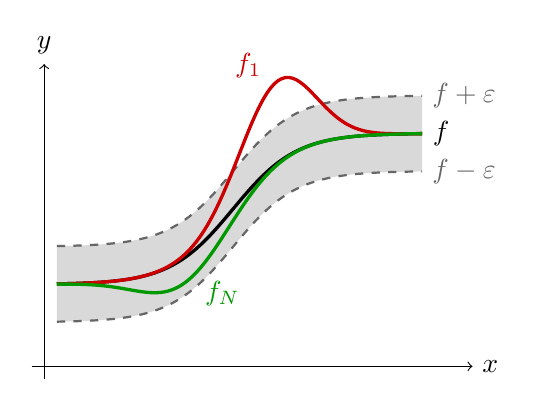
\begin{tikzpicture}[
        declare function={
            % Removed the rogue deg() - tanh takes standard real numbers!
            f(\x) = 2.5 + 1.2*tanh(\x - 3);
            % f_1 breaks outside the upper bound
            f1(\x) = f(\x) + 1.3*exp(-1.5*(\x-3.7)*(\x-3.7));
            % f_N stays inside the epsilon tube
            fN(\x) = f(\x) - 0.4*exp(-1.2*(\x-2.2)*(\x-2.2));
            % Renamed to avoid colliding with pgfmath's internal machine epsilon
            myeps = 0.6;
        },
        scale=0.8
    ]
        % Axes
        \draw[->] (-0.2, 0) -- (6.8, 0) node[right] {$x$};
        \draw[->] (0, -0.2) -- (0, 4.8) node[above] {$y$};
    
        % Shaded Epsilon Tube
        \fill[gray!30] 
            plot[domain=0.2:6, samples=100] (\x, {f(\x) + myeps})
            -- plot[domain=0.2:6, samples=100] ({6.2-\x}, {f(6.2-\x) - myeps})
            -- cycle;
    
        % Tube boundaries
        \draw[dashed, gray!80!black, thick] plot[domain=0.2:6, samples=100] (\x, {f(\x) + myeps}) node[right] {$f + \varepsilon$};
        \draw[dashed, gray!80!black, thick] plot[domain=0.2:6, samples=100] (\x, {f(\x) - myeps}) node[right] {$f - \varepsilon$};
    
        % Limit Function f
        \draw[very thick, black] plot[domain=0.2:6, samples=100] (\x, {f(\x)}) node[right] {$f$};
    
        % Function f_1 (Red)
        \draw[very thick, red!80!black] plot[domain=0.2:6, samples=100] (\x, {f1(\x)});
        \node[red!80!black, above left] at (3.6, {f1(3.6)}) {$f_1$};
    
        % Function f_N (Green)
        \draw[very thick, green!60!black] plot[domain=0.2:6, samples=100] (\x, {fN(\x)});
        \node[green!60!black, below right] at (2.4,1.5) {$f_N$};
    
    \end{tikzpicture}
\end{center}

\begin{exercise*}
    Prove that uniform convergence implies pointwise convergence.
\end{exercise*}
As hinted at in the discussion of pointwise convergence, we may restate the definition of uniform convergence in terms of the supremum norm (which is perhaps a more intuitive way of thinking about the concept):
\begin{lemma}
    \begin{shaded*}
        Let $f_n:D\to\R$ be a sequence of functions on $D$. Then
        \[f_n\rightrightarrows f \iff \lim_{n\to\infty}\|f_n-f\|_\infty = 0.\]
    \end{shaded*}
\end{lemma}
\begin{proof}
    Exercise.
\end{proof}
In other words, the maximum error between the function $f_n$ and $f$ goes to zero \textit{uniformly} in the domain $D$ (i.e. independent of where the function is evaluated in the domain), which intuitively means the functions $f_n$ are being ``squeezed'' together towards the limit function across the whole domain. In this sense, properties like continuity of the limit functions should be preserved in the limit as no ``tearing'' can take place, unlike in pointwise convergence (we will prove these facts in the next subsection). The idea is demonstrated below with the functions $f:[0,2\pi]\to\R$ defined by $f_n(x)=\frac{\sin x}{n}$ for $n\ge 1$. Since $\sin x$ is uniformly bounded by $-1$ and $1$ on $[0,2\pi]$, we have $f_n\rightrightarrows 0$: 
\begin{center}
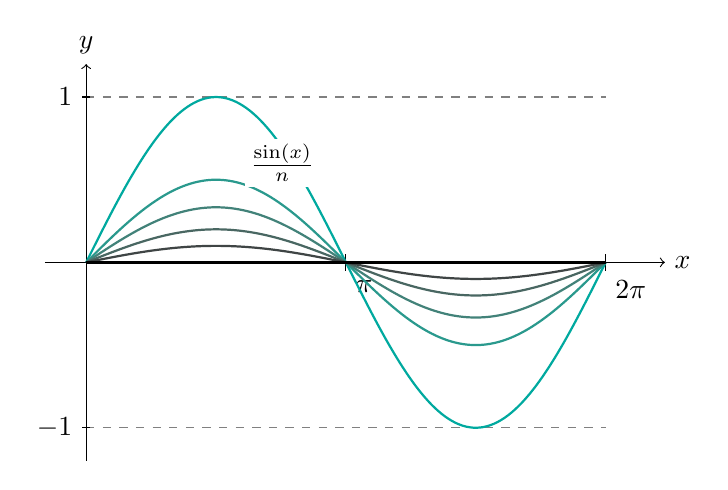
\begin{tikzpicture}[x=1.5cm, y=3cm, scale=0.7]
    % Axes
    \draw [->] (-0.5, 0) -- (7, 0) node [right] {$x$};
    \draw [->] (0, -1.2) -- (0, 1.2) node [above] {$y$};
  
    % Dashed bounds to visualize the uniform bound (supremum norm)
    \draw [dashed, gray] (0, 1) -- (2*pi, 1);
    \draw [dashed, gray] (0, -1) -- (2*pi, -1);
  
    % Ticks
    \draw (pi, 0.05) -- (pi, -0.05) node [below right] {$\pi$};
    \draw (2*pi, 0.05) -- (2*pi, -0.05) node [below right] {$2\pi$};
    \draw (0.05, 1) -- (-0.05, 1) node [left] {$1$};
    \draw (0.05, -1) -- (-0.05, -1) node [left] {$-1$};
  
    \begin{scope}
      % Sequence of functions f_n(x) = sin(x)/n
      % \i controls color shading, \n is the denominator
      \foreach \i/\n in {
        0/1, 
        1/2, 
        2/3, 
        3/5, 
        4/10
      } {
        % Shading: 100 is pure green, decreasing towards 0 (black)
        \pgfmathsetmacro\c{100 - 20 * \i};
        
        % Note: '\x r' converts radians to degrees for pgfmath's sin()
        \draw [domain=0:2*pi, samples=150, Emerald!\c!black, thick] 
          plot (\x, {sin(\x r) / \n});
      }
    \end{scope}
  
    % Limit function f(x) = 0 emphasized over the x-axis
    \draw [very thick, black] (0, 0) -- (2*pi, 0);
  
    % Single label for the functions
    \node [fill=white, inner sep=2pt] at (pi/2 + 0.8, 0.6) {$\frac{\sin(x)}{n}$};
  
  \end{tikzpicture}
\end{center}
In this example, since the limit function is also 0, this graph also visualises how the error $\|f_n-f\|_\infty \to 0$ as $n\to\infty$ uniformly across the whole domain.

\subsection{Properties of Uniform Convergence}
\begin{theorem}
\label{thm:ucc}
    \begin{shaded*}
        If $f_n\rightrightarrows f$ on $[a,b]$ and each $f_n$ is continuous on $[a,b]$ then $f$ is continuous on $[a,b]$.
    \end{shaded*}
\end{theorem}
\begin{proof}
    We will show that $f$ is uniformly continuous on $[a,b]$. Let $\varepsilon$ be arbitrary. By uniform convergence, there exists $N\in\N$ such that for all $n\ge N$, $|f(t)-f_n(t)|<\frac{\varepsilon}{3}$ for all $t\in[a,b]$.

    Since $f_N$ is continuous on a compact interval $[a,b]$, it is uniformly continuous on $[a,b]$ so there exists $\delta=\delta(N,\varepsilon)$ such that for all $s,t\in [a,b]$, $|s-t|<\delta\implies |f_N(s)-f_N(t)|<\frac{\varepsilon}{3}$.
    
    Therefore, if $x,y\in[a,b]$ are such that $|x-y|<\delta$, we have
    \begin{align*}
        |f(x)-f(y)|&=|f(x)-f_N(x)+f_N(x)-f_N(y)+f_N(y)-f(y)|\\
        &\le |f(x)-f_N(x)|+|f_N(x)-f_N(y)|+|f_N(y)-f(y)|\\
        &< \frac{\varepsilon}{3}+\frac{\varepsilon}{3}+\frac{\varepsilon}{3}\\
        &=\varepsilon.
    \end{align*}
Thus, $f$ is uniformly continuous on $[a,b]$, so in particular $f$ is continuous on $[a,b]$.\qedhere
\end{proof}

\begin{theorem}
\label{thm:unifintegral}
    \begin{shaded*}
        If $f_n\rightrightarrows f$ on $[a,b]$ and $f_n$ are integrable on $[a,b]$ then $f$ is integrable and
        \[\int_a^b f(x)\d{x}=\lim_{n\to\infty}\int _a^b f_n(x)\d{x}.\]
    \end{shaded*}
\end{theorem}
\begin{proof}
    We will first show that $f$ is integrable using the $\varepsilon$-criterion for (Darboux) integrability (Theorem \ref{thm:epsilonintegrability}). First we must check that $f$ is bounded: since $f_n$ is integrable on $[a,b]$ for each $n\in\N$, each $f_n$ must be bounded and by uniform convergence there exists $N\in\N$ such that $\|f_n-f\|_\infty <1.$ Then for all $x\in[a,b]$ we have \[|f(x)|\le |f(x)-f_N(x)|+|f_N(x)|<1+|f_N(x)|,\]
    so $f$ is bounded. 
    
    Now, let $\varepsilon>0$ be arbitrary. By uniform convergence fix $n$ sufficiently large such that \[\|f_n-f\|_\infty <\frac{\varepsilon}{4(b-a)}.\]
    Since $f_n$ is integrable, by Theorem \ref{thm:epsilonintegrability} there exists a partition $P=\{x_0,\dots,x_n\}$ of $[a,b]$ such that \[U(f_n,P)-L(f_n,P)<\frac{\varepsilon}{2}.\]
    For each subinterval $[x_{i - 1},x_i]$, where $1\le i\le n$, we write 
    \[m^n_i=\inf_{x\in [x_{i - 1},x_i]}f_n(x)\quad\text{and}\quad M^n_i=\sup_{x\in[x_{i - 1},x_i]}f_n(x),\]
    and the usual notation $m_i,M_i$ for the function $f$. Our goal is now to bound the oscillation of $f$, $M_i-m_i$, by $f_n$'s oscillation, plus some error term, which we will achieve by using the uniform convergence of $f_n$ to $f$. From the uniform convergence bound above, for every $x\in[a,b]$ we have \[f_n(x)-\frac{\varepsilon}{4(b-a)}<f(x)<f_n(x)+\frac{\varepsilon}{4(b-a)},\]
    and using standard properties of suprema and infima, taking $\sup$ and $\inf$ over these inequalities yields \[m_i\ge m_i^n-\frac{\varepsilon}{4(b-a)}\quad\text{and}\quad M_i\le M_i^n+\frac{\varepsilon}{4(b-a)},\]
    from which it follows that \[M_i-m_i\le M^n_i-m^n_i+\frac{\varepsilon}{2(b-a)}.\]
    Summing this inequality over all $1\le i\le n$, we get
    \begin{align*}
        U(f,P)-L(f,P)&=\sum_{i=1}^n(M_i-m_i)(x_i-x_{i - 1})\\
        &\le \sum_{i=1}^n(M^n_i-m^n_i+)(x_i-x_{i - 1})+\sum_{i=1}^n\frac{\varepsilon}{2(b-a)}(x_i-x_{i - 1})\\
        &= U(f_n,P)-L(f_n,P)+\frac{\varepsilon}{2}\\
        &<\frac{\varepsilon}{2}+\frac{\varepsilon}{2}\\
        &=\varepsilon,
    \end{align*}
    so $f$ is integrable on $[a,b]$ by Theorem \ref{thm:epsilonintegrability}.

    To show the integral equality, using standard properties of the integral, we have for $n\in\N$
    \begin{align*}
        \left|\int_a^b f_n(x)\d{x}-\int_a^b f(x)\d{x}\right|&=\left|\int_a^b (f_n(x)-f(x))\d{x}\right|\\
        &\le \int_a^b |f_n(x)-f(x)|\d{x}\\
        &\le (b-a)\|f_n-f\|_\infty,
    \end{align*}
    so since $\|f_n-f\|_\infty\to 0$ by uniform convergence of $f_n$ to $f$, and $(b-a)$ is finite, this upper bound can be made arbitrarily small for sufficiently large $n$, so by definition of sequence convergence (Definition \ref{def:convergence1}), we have \[\lim_{n\to\infty}\int_a^b f_n(x)\d{x}=\int_a^b f(x)\d{x}.\]\qedhere
\end{proof}

\begin{example}
    We can use Theorem \ref{thm:unifintegral} to evaluate limits of integrals that would otherwise be computationally tedious. Consider the sequence of functions on the closed interval $[0,1]$:
    \[
        f_n(x) = \frac{x}{1 + nx^2}.
    \]
    First, we find the pointwise limit. For $x = 0$, $f_n(0) = 0$ for all $n$. For any fixed $x \in (0,1]$, the denominator grows linearly with $n$, so $\lim_{n \to \infty} f_n(x) = 0$. Thus, $f_n \to 0$ pointwise.
    
    To apply Theorem \ref{thm:unifintegral}, we must verify that this convergence is \textit{uniform}. We find the maximum of $f_n(x)$ using standard calculus:
    \[
        f_n'(x) = \frac{(1+nx^2) - x(2nx)}{(1+nx^2)^2} = \frac{1 - nx^2}{(1+nx^2)^2}.
    \]
    Setting the derivative to zero yields a critical point at $x = 1/\sqrt{n}$; to confirm this is the global maximum on $[0,1]$, observe the sign of the derivative: for $0 \le x < 1/\sqrt{n}$, we have $1 - nx^2 > 0$, so $f_n'(x) > 0$ (the function is strictly increasing). For $x > 1/\sqrt{n}$, we have $1 - nx^2 < 0$, so $f_n'(x) < 0$ (the function is strictly decreasing). 
    
    Because $f_n$ strictly increases to this point and strictly decreases away from it, the critical point is the maximum (first derivative test). Therefore, evaluating the function here gives the supremum:
    \[
        \|f_n - 0\|_\infty = f_n\left(\frac{1}{\sqrt{n}}\right) = \frac{1/\sqrt{n}}{1 + 1} = \frac{1}{2\sqrt{n}}.
    \]
    Because $\lim_{n \to \infty} \frac{1}{2\sqrt{n}} = 0$, the sequence converges uniformly to the zero function ($f_n \rightrightarrows 0$).
    
    By Theorem \ref{thm:unifintegral}, we are now mathematically guaranteed that the limit of the integrals is the integral of the limit:
    \[
        \lim_{n \to \infty} \int_0^1 \frac{x}{1 + nx^2} \d{x} = \int_0^1 0 \d{x} = 0.
    \]
     We can verify this by integrating the sequence directly. Using the substitution $u = 1+nx^2$ (with the change of variables theorem for integrals from a previous exercise), we get
    \[
        \int_0^1 \frac{x}{1 + nx^2} \d{x} = \left[ \frac{\ln(1+nx^2)}{2n} \right]_0^1 = \frac{\ln(1+n)}{2n}.
    \]
    By L'H\^{o}pital's rule (or comparing growth rates), $\lim_{n \to \infty} \frac{\ln(1+n)}{2n} = 0$, which indeed matches the theorem's prediction.
\end{example}


\begin{example}
    It is also instructive to see what can go wrong when the hypothesis of uniform convergence fails. Consider the sequence of functions $g_n:[0,1]\to\R$ defined by
    \[
        g_n(x) = n x (1-x^2)^n.
    \]
    For $x=0$, $g_n(0) = 0$. For any $x \in (0,1]$, the term $(1-x^2)$ is strictly between $0$ and $1$. Because exponential decay dominates polynomial growth, $\lim_{n \to \infty} n x (1-x^2)^n = 0$. Thus, $g_n$ converges pointwise to the zero function.
    \begin{center}
    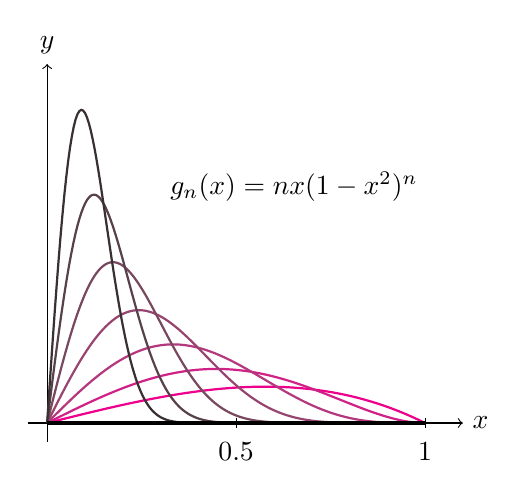
\begin{tikzpicture}[x=8cm, y=2cm, scale = 0.6]
        % Axes
        \draw [->] (-0.05, 0) -- (1.1, 0) node [right] {$x$};
        \draw [->] (0, -0.2) -- (0, 3.8) node [above] {$y$};
      
        \begin{scope}
          \clip (-0.05, -0.2) rectangle (1.1, 3.6);
      
          % Sequence of functions g_n(x) = n*x*(1-x^2)^n
          % \i controls color shading, \n is the parameter
          \foreach \i/\n in {
            0/1, 
            1/2, 
            2/4, 
            3/8, 
            4/16, 
            5/32, 
            6/60
          } {
            % Shading: 100 is pure magenta, decreasing towards 10 (very dark magenta)
            \pgfmathsetmacro\c{100 - 15 * \i};
            
            \draw [domain=0:1, samples=200, magenta!\c!black, thick] 
              plot (\x, {\n * \x * (1 - \x*\x)^\n});
          }
        \end{scope}
      
        % Ticks
        \draw (1, 0.05) -- (1, -0.05) node [below=2pt] {$1$};
        \draw (0.5, 0.05) -- (0.5, -0.05) node [below=2pt] {$0.5$};
        
        % Limit function f(x) = 0
        \draw [very thick, black] (0, 0) -- (1, 0);
        
        % Function Label
        \node [right, align=left] at (0.3, 2.5) {$g_n(x) = n x (1-x^2)^n$};
      
      \end{tikzpicture}
    \end{center}
    
    If we naively interchange the limit and the integral, we would expect the area to be $0$. Let us explicitly compute the integral using the substitution $u = 1-x^2$ (again using the change of variables theorem for integrals from a previous exercise):
    \[
        \int_0^1 n x (1-x^2)^n \d{x} = \frac{n}{2} \int_0^1 u^n \d{u} = \frac{n}{2} \left[ \frac{u^{n+1}}{n+1} \right]_0^1 = \frac{n}{2(n+1)}.
    \]
    Taking the limit as $n \to \infty$ yields:
    \[
        \lim_{n \to \infty} \int_0^1 g_n(x) \d{x} = \lim_{n \to \infty} \frac{n}{2n+2} = \frac{1}{2}.
    \]
    The limit of the integrals ($1/2$) does \textit{not} equal the integral of the limit ($0$). 
    
    This failure occurs because the convergence $g_n \to 0$ is pointwise, not uniform. As $n$ increases, the function forms an increasingly thin ``spike'' of area converging to $1/2$ that slides towards $x=0$. While the spike eventually passes any fixed point $x > 0$ (causing the pointwise limit to be $0$), its maximum height grows towards infinity, violating the uniform bound required by Theorem \ref{thm:unifintegral}, thereby allowing the area, $\int_0^1 g_n$, in the limit as $n\to\infty$ to be non-zero (one can think of this as a balance between $x\to 0$ and the height going to infinity, settling on a finite number, $1/2$; indeed, this is represented in the formula for the area, $\frac{n}{2n+2}$).
\end{example}

One may wonder whether differentiability of the sequence functions passes to the limit function when convergence is uniform. With some extra hypotheses this is true, however uniform convergence of the sequence of \textit{derivatives} is required, rather than just uniform convergence of the original differentiable functions.

One way to see why this theorem does not work without uniform convergence of the derivatives is that sharp corners (where a function is not differentiable because the left and right slopes exist, but are not equal) can be ``\textit{smoothed out}'' by sequences of functions, all of which are differentiable everywhere. The following example makes this clear.

\begin{example}
    Consider the sequence of functions $g_n:[-1,1] \to \R$ defined by
    \[
        g_n(x) = \sqrt{x^2+\frac{1}{n}}.
    \]

    \begin{center}
        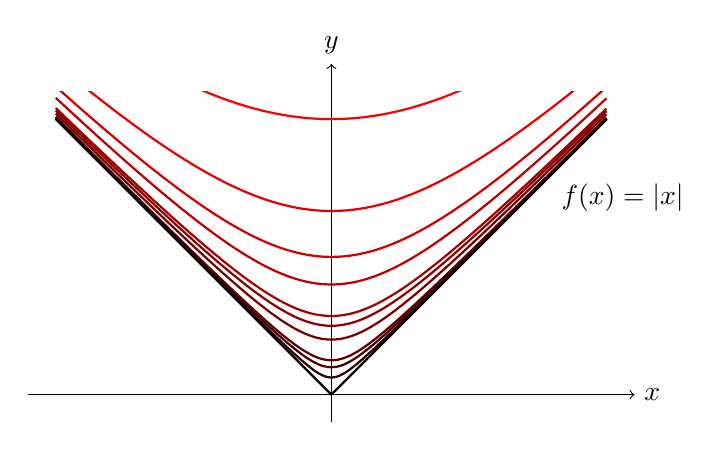
\begin{tikzpicture}[x=10cm, y=10cm, scale=0.7]
            % Axes
            \draw [->] (-0.55, 0) -- (0.55, 0) node [right] {$x$};
            \draw [->] (0, -0.05) -- (0, 0.6) node [above] {$y$};
          
            \begin{scope}
              \clip (-0.55, -0.05) rectangle (0.55, 0.55);
          
              % Sequence of functions g_n(x) = sqrt(x^2 + 1/n)
              \foreach \i/\n in {
                0/4, 
                1/9, 
                2/16, 
                3/25, 
                4/49, 
                5/64, 
                6/100, 
                7/256, 
                8/400, 
                9/1024
              } {
                % Shading: 100 is pure red, decreasing towards 19 (dark red/black)
                \pgfmathsetmacro\c{100 - 9 * \i};
                
                \draw [domain=-0.5:0.5, samples=200, red!\c!black, thick] 
                  plot (\x, {sqrt(\x*\x + 1/\n)});
              }
            \end{scope}
          
            % Limit function f(x) = |x|
            \draw [thick, black] (0, 0) -- (0.5, 0.5);
            \draw [thick, black] (0, 0) -- (-0.5, 0.5);
            \node [below right] at (0.4, 0.4) {$f(x) = |x|$};
          
          \end{tikzpicture}
    \end{center}

    Every function in this sequence is continuously differentiable everywhere with \[g'_n(x)=\frac{x}{\sqrt{x^2+\frac{1}{n}}},\]
    for each $x\in[-1,1]$.

    We claim that $g_n\rightrightarrows g$ where $g:[-1,1]\to\R$ is defined by $g(x)=|x|$. Indeed, for every $x\in[-1,1]$ and $n\ge 1$ we have
    \[0\le g_n(x)-g(x)=\sqrt{x^2+\frac{1}{n}}-|x|=\frac{1}{n}{\sqrt{x^2+\frac{1}{n}}+|x|}\le \frac{1/n}{1/\sqrt{n}}=\frac{1}{\sqrt{n}},\]
    so taking the supremum over $[-1,1]$ we get, for each $n\ge 1$,
    \[\|g_n-g\|_\infty \le\frac{1}{\sqrt{n}},\]
    and $1/\sqrt{n}\to 0$ as $n\to\infty$, so $g_n\rightrightarrows g$.
    
    This demonstrates that a uniform limit of differentiable functions need not be differentiable.
\end{example}

\begin{example}
    Even in cases where the uniform limit function remains differentiable, its derivative may have no relationship to the derivatives of the original sequence (i.e. the limit may not commute with the derivative). Let $f_n:[0,1] \to \R$ be defined by
    \[
        f_n(x) = \frac{\sin(n^2 x)}{n}.
    \]

    \begin{center}
    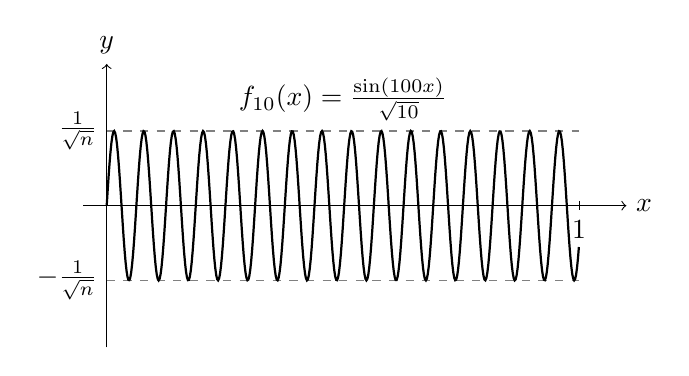
\begin{tikzpicture}[x=10cm, y=5cm, scale=0.6]
        % Axes
  \draw [->] (-0.05, 0) -- (1.1, 0) node [right] {$x$};
  \draw [->] (0, -0.6) -- (0, 0.6) node [above] {$y$};

  % Ticks and Uniform Bounds
  \draw [dashed, gray] (0, {1/sqrt(10)}) -- (1, {1/sqrt(10)});
  \draw [dashed, gray] (0, {-1/sqrt(10)}) -- (1, {-1/sqrt(10)});
  \draw (1, 0.02) -- (1, -0.02) node [below] {$1$};
  
  % y-axis labels
  \node [left] at (0, {1/sqrt(10)}) {$\frac{1}{\sqrt{n}}$};
  \node [left] at (0, {-1/sqrt(10)}) {$-\frac{1}{\sqrt{n}}$};

  \begin{scope}
    \clip (-0.05, -0.55) rectangle (1.1, 0.55);

    % The highly oscillatory function for n=10
    % n^2 = 100. We use 500 samples to ensure the high-frequency waves render smoothly.
    % \x r converts radians to degrees for pgfmath
    \draw [domain=0:1, samples=500,thick] 
      plot (\x, {sin(100 * \x r) / sqrt(10)});
  \end{scope}

  % Function Label
  \node [fill=white, inner sep=2pt] at (0.5, 0.45) {$f_{10}(x) = \frac{\sin(100x)}{\sqrt{10}}$};

\end{tikzpicture}
    \end{center}

    Because $|\sin(n^2 x)| \le 1$, the amplitude of these functions is bounded by $1/n$, meaning $f_n$ converges uniformly to the identically zero function, $f(x) = 0$. This limit function is trivially differentiable everywhere, with $f'(x) = 0$.
    
    However, if we examine the sequence of derivatives, we find $f_n'(x) = n \cos(n^2 x)$. Evaluated at the origin, $f_n'(0) = n$, which diverges to infinity as $n \to \infty$. Thus, $\lim_{n \to \infty} f_n'(x) \neq f'(x)$. 
    
    This pathological example shows that uniform convergence controls only the amplitude of the functions (to be uniformly within $\varepsilon$ of the limit function, past some point $N\in\N$), not their slopes. The functions $f_n$, in this case, are uniformly squeezed to zero while the increasing oscillations lead to unbounded slopes.
\end{example}

Hence, in order to guarantee that a limit function is differentiable, and to safely commute the limit and derivative operations, we require a stronger theorem.


\begin{theorem}
\label{thm:unifderivative}
    \begin{shaded*}
        Let $f_n \colon \lbrack a,b \rbrack \to \R$ be a sequence of continuously differentiable functions. Assume that:
        \begin{enumerate}
            \item The sequence of derivatives $f_n'$ converges uniformly to a function $g$ on $\lbrack a,b \rbrack$.
            \item There exists at least one point $x_0 \in \lbrack a,b \rbrack$ such that the sequence of numbers $f_n(x_0)$ converges in $\R$.
        \end{enumerate}
        Then there exists a function $f$ such that $f_n \to f$ uniformly on $\lbrack a,b \rbrack$, and
        \[
            f'(x) = g(x) \quad \text{for all } x \in (a,b).
        \]
        In particular, $f$ is differentiable and $f'(x) = \lim_{n \to \infty} f_n'(x)$ for all $x \in (a,b)$.
    \end{shaded*}
\end{theorem}
\begin{proof}
    Since each $f_n$ is continuously differentiable on $\lbrack a,b \rbrack$, the Fundamental Theorem of Calculus gives
    \[
        f_n(x) = f_n(x_0) + \int_{x_0}^x f_n'(t) \d{t}
    \]
    for all $x \in \lbrack a,b \rbrack$. By hypothesis, the sequence of real numbers $(f_n(x_0))$ converges to some limit $L$, and $f_n' \to g$ uniformly. Because each $f_n'$ is continuous and converges uniformly to $g$, the limit function $g$ must also be continuous, and therefore integrable on $\lbrack a,b \rbrack$. We may thus define our candidate limit function $f \colon \lbrack a,b \rbrack \to \R$ as
    \[
        f(x) \coloneqq L + \int_{x_0}^x g(t) \d{t}.
    \]
    By the Fundamental Theorem of Calculus (Theorem \ref{thm:ftc1}), since $g$ is continuous (as a uniform limit of continuous functions), $f$ is differentiable and $f'(x) = g(x)$ for all $x \in (a,b)$.
    
    It remains to prove that $f_n \to f$ uniformly on $\lbrack a,b \rbrack$. For any $x \in \lbrack a,b \rbrack$, we evaluate the difference
    \[
        |f_n(x) - f(x)| = \left| f_n(x_0) - L + \int_{x_0}^x (f_n'(t) - g(t)) \d{t} \right|.
    \]
    Applying the triangle inequality and bounding the integral by the supremum norm of the integrand yields
    \begin{align*}
        |f_n(x) - f(x)| &\le |f_n(x_0) - L| + \left| \int_{x_0}^x |f_n'(t) - g(t)| \d{t} \right|\\
        &\le |f_n(x_0) - L| + \|f_n' - g\|_\infty |x - x_0|.
    \end{align*}
    Since $|x - x_0| \le b-a$ for all $x \in \lbrack a,b \rbrack$, taking the supremum over the interval gives
    \[
        \|f_n - f\|_\infty \le |f_n(x_0) - L| + (b-a)\|f_n' - g\|_\infty.
    \]
    As $n \to \infty$, we have $f_n(x_0) \to L$ and $\|f_n' - g\|_\infty \to 0$. Therefore, $\|f_n - f\|_\infty \to 0$, which proves that $f_n$ converges uniformly to $f$ on $\lbrack a,b \rbrack$.
\end{proof}

\begin{remark}
    The key idea in the proof is the Fundamental Theorem of Calculus (Theorem \ref{thm:ftc1}), which allows us to reconstruct a function globally from a single starting value and its rate of change by integration. 
    
    The point $x_0$ acts as an ``anchor'' to guarantee the existence of a limit function; because $f_n(x_0)$ converges, this pins the sequence down and prevents the functions from simply drifting vertically to infinity (for example, without this hypothesis the sequence of constant functions $f_1=1,f_2=2,\dots$ have derivatives which converge uniformly to the zero function, but $f_n$ does not converge to any function). From this point $x_0$, we integrate the derivatives $f_n'$ outwards to build the rest of the function $f_n$, and we are guaranteed that there exists a limit function with the properties we desire by uniform convergence.
\end{remark}

\begin{exercise*}
    Show that if $f_n\to f$ and $g_n\to g$ uniformly on $[a,b]$, and $f_n,g_n$ are all continuous, then $f_ng_n\to fg$.
\end{exercise*}



\end{document}

